The city of Brisbane has been taken over by large mutated wombats, and you must lead the people to safety.

The roads in Brisbane are laid out in a large grid. There are $R$ horizontal roads that run east­to­west, numbered $0, \dots, (R ­- 1)$ in order from north to south, and $C$ vertical roads that run north­to­south, numbered $0, \dots, (C ­- 1)$ in order from west to east, as shown in the picture below.

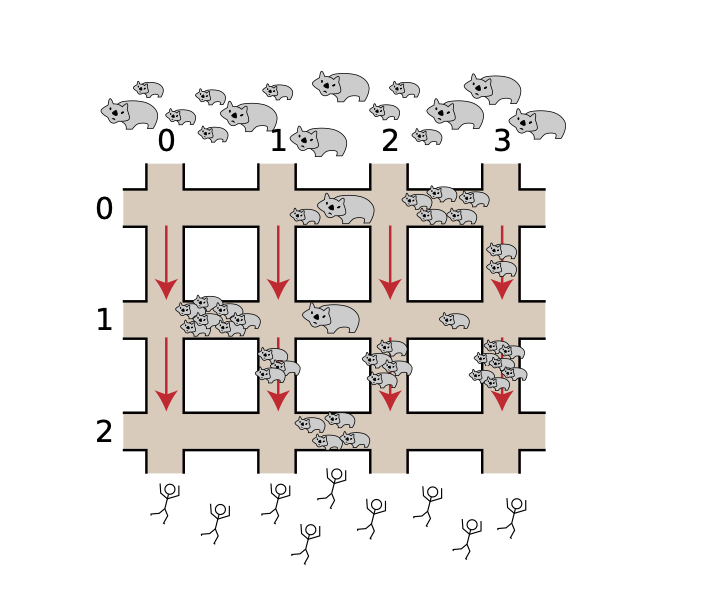
\includegraphics{wombats1.png}

The wombats have invaded from the north, and the people are escaping to the south. People can run along horizontal roads in either direction, but on vertical roads they will \textit{only run towards the south}, towards safety.

The intersection of horizontal road $P$ with vertical road $Q$ is denoted $(P, Q)$. Each segment of road between two intersections contains some number of wombats, and these numbers may change over time. Your task is to guide each person from some given intersection in the north (on horizontal road $0$) to some given intersection in the south (on horizontal road $(R ­- 1)$), taking them on a route that passes as few wombats as possible.

To begin, you will be given the size of the grid and the number of wombats on each road segment. Following this you will be given a series of $E$ events, each of which is either:
                      
\begin{itemize}
\item a \textit{change}, which alters the number of wombats on some road segment; or
\item an \textit{escape}, where some person arrives at a given intersection on horizontal road $0$, and you must find a route to a given intersection on horizontal road $(R -­ 1)$ that passes the fewest possible wombats.
\end{itemize}

You must handle these events by implementing the routines \t{init()}, \t{changeH()}, \t{changeV()} and \t{escape()}, as described below.

You should submit a file implementing the procedures \t{init()}, \t{changeH()} and \t{changeV()} and the function \t{escape()}.

Your Procedure \t{init()}:

\t{void init(int R, int C, int H[5000][200], int V[5000][200]);}

This procedure gives you the initial layout of the map, and allows you to initialise any global variables and data structures. It will be called only once, before any calls to
\t{changeH()}, \t{changeV()} or \t{escape()}. 

Parameters:
\begin{itemize}
\item $R$: The number of horizontal roads.
\item $C$: The number of vertical roads.
\item $H$: A two­dimensional array of size $R \cdot (C ­- 1)$, where $H[P][Q]$ gives the number of wombats on the segment of horizontal road between intersections $(P, Q)$ and $(P, Q + 1)$.
\item $V$: A two­dimensional array of size $(R ­- 1) \cdot C$, where $V[P][Q]$ gives the number of wombats on the segment of vertical road between intersections $(P, Q)$ and $(P + 1, Q)$.
\end{itemize}

Your Procedure \t{changeH()}:

\t{void changeH(int P, int Q, int W);}

This procedure will be called when the number of wombats changes on the horizontal road segment between intersections $(P, Q)$ and $(P, Q + 1)$.

Parameters:
\begin{itemize}
\item $P$: Indicates which horizontal road is affected $(0 \leq P \leq R ­- 1)$.
\item $Q$: Indicates between which two vertical roads the segment lies $(0 \leq Q \leq C ­- 2)$.
\item $W$: The new number of wombats on this road segment $(0 \leq W \leq 1,000)$.
\end{itemize}



Your Procedure: \t{changeV()}:

\t{void changeV(int P, int Q, int W);}

This procedure will be called when the number of wombats changes on the vertical road segment between intersections $(P, Q)$ and $(P + 1, Q)$.

Parameters:
\begin{itemize}
\item $P$: Indicates between which two horizontal roads the segment lies $(0 \leq P \leq R -­ 2)$
\item $Q$: Indicates which vertical road is affected $(0 \leq Q \leq C -­ 1)$.
\item $W$: The new number of wombats on this road segment $( 0 \leq W \leq 1\,000)$.
\end{itemize}


            
Your Function \t{escape()}:

\t{int escape(int V1, int V2);}

This function should calculate the fewest possible wombats a person must pass when travelling from intersection $(0, V1)$ to $(R­1, V2)$.

Parameters:
\begin{itemize}
\item $V1$: Indicates where the person begins on horizontal row $0$ $( 0 \leq V1 \leq C­-1 )$.
\item $V2$: Indicates where the person ends on horizontal row $R-­1$ $( 0 \leq V2 \leq C­-1 )$.
\item \textit{Returns}: The smallest number of wombats the person must pass.
\end{itemize}
